\pdfbookmark{Общая характеристика работы}{characteristic}             % Закладка pdf
\section*{Общая характеристика работы}
\newcommand{\actuality}{\pdfbookmark[1]{Актуальность}{actuality}\underline{\textbf{\actualityTXT}}}
\newcommand{\progress}{\pdfbookmark[1]{Разработанность темы}{progress}\underline{\textbf{\progressTXT}}}
\newcommand{\aim}{\pdfbookmark[1]{Цели}{aim}\underline{{\textbf\aimTXT}}}
\newcommand{\tasks}{\pdfbookmark[1]{Задачи}{tasks}\underline{\textbf{\tasksTXT}}}
\newcommand{\aimtasks}{\pdfbookmark[1]{Цели и задачи}{aimtasks}\aimtasksTXT}
\newcommand{\compliance}{\pdfbookmark[1]{Соответствие паспорту специальности}{compliance}\underline{\textbf{\complianceTXT}}}
\newcommand{\novelty}{\pdfbookmark[1]{Научная новизна}{novelty}\underline{\textbf{\noveltyTXT}}}
\newcommand{\influence}{\pdfbookmark[1]{Практическая значимость}{influence}\underline{\textbf{\influenceTXT}}}
\newcommand{\methods}{\pdfbookmark[1]{Методология и методы исследования}{methods}\underline{\textbf{\methodsTXT}}}
\newcommand{\defpositions}{\pdfbookmark[1]{Положения, выносимые на защиту}{defpositions}\underline{\textbf{\defpositionsTXT}}}
\newcommand{\reliability}{\pdfbookmark[1]{Достоверность}{reliability}\underline{\textbf{\reliabilityTXT}}}
\newcommand{\probation}{\pdfbookmark[1]{Апробация}{probation}\underline{\textbf{\probationTXT}}}
\newcommand{\contribution}{\pdfbookmark[1]{Личный вклад}{contribution}\underline{\textbf{\contributionTXT}}}
\newcommand{\publications}{\pdfbookmark[1]{Публикации}{publications}\underline{\textbf{\publicationsTXT}}}


{\actuality}
Индустрия создания программного обеспечения (далее - ПО) растет очень быстрыми темпами. Согласно отчету компании Gartner, в 2022 году глобальный рынок ПО оценивался в 4.534 милли­ арда долларов США, что на 3\% больше, чем в 2021 году. Ожидается, что рост индустрии будет продолжаться и в ближайшие годы. Рост инду­стрии ПО обусловлен многими факторами. Прежде всего, сегодня ПО используется в различных отраслях, от банковского и финансового секторов до здравоохранения и государственного управления. При этом появляются новые технологии и требования, что приводит к со­зданию новых программных продуктов и услуг. Также следует отметить, что развитие интернета, мобильных устройств и облачных технологий создает новые возможности для создания и использования ПО. Более того, в условиях пандемии COVID-19 большое количество людей перешло на удаленную работу, что привело к росту спроса на ПО для удаленной работы. Развитие индустрии создания ПО требует повышения эффективность разработки новых программных продуктов и при этом предъявляет всё большие требования к их безопасности и качеству.

В настоящее время проблема обеспечения информационной безопасности в государственных и коммерческих автоматизированных системах обработки и управления информацией встаёт особенно остро. Среди основных причин этого: политическая нестабильность и стремительно возрастающий объем информатизации в мире, а также совершенствование и повсеместная популяризация компьютерных технологий, в том числе приводящая к существенному росту числа и навыков потенциальных нарушителей – формированию «армии» хакеров, зачастую действующих из коростных побуждений, в том числе в рамках кибер-операций, проводимых в интересах различных государств. Экспертные оценки прогнозируют трехкратный рост финансовых потерь от киберпреступности в ближайшие пять лет , при этом угрозы устойчивости государственных систем не поддаются исчислению, поскольку несут в себе риски функционирования государства как целостной сущности.
Современные программные системы по оценке например НИУ ВШЭ «в 98\% случаев содержат в себе open source, или открытое (свободное) ПО. При этом программы в среднем на 75\% состоят из open source компонентов». Существующее обывательское представление от том, что свободное ПО является по определению более доверенным, а следовательно – безопасным в использовании, в общем случае не является верным. Действительно, обнаружение потенциальных вредоносных «закладок» и недекларированных возможностей в проприетарном программном обеспечении, поставляемом пользователю в бинарном и/или обмундированном виде, представляет собой проблему, которая по определению отсутствует при использовании открытого ПО. Однако, вместе с тем, проприетарное ПО как правило является источником дохода разрабатывающей его компании, а следовательно существует организация (как минимум одна), непосредственно заинтересованная в положительной репутации ПО, а следовательно – отсутствии в нём публично известных (как минимум – публично-обнаруживаемых) НДВ, а также минимизации числа различных уязвимостей (архитектурных, конфигурационных, кодовых, вносимых сборочной системой).

В программировании программные библиотеки позволяют повторно использовать код, уменьшать объем работы разработчиков и сокращать время разработки программных продуктов. Программная библиотека (далее библиотека) представляет собой набор предварительно написанного кода, который можно использовать для добавления определенных функций в программное приложение. Она является своего рода строительным блоком для разработки  ПО, предоставляя разработчикам возможность повторно использовать код и экономить время.
Библиотеки могут включать в себя широкий спектр сущностей: функции, классы, структуры, перечисления и т. д.. Как правильно они разрабатываются так, чтобы их было легко использовать и интегрировать в существующее приложение, что позволяет разработчикам быстро и эффективно добавлять новые функции и возможности.
Использование программных библиотек может значительно улучшить процесс разработки за счет уменьшения объема кода, который необходимо писать с нуля. Это может привести к сокращению времени разработки, улучшению качества кода и снижению затрат на разработку. Кроме того, библиотеки могут быть общими и использоваться несколькими разработчиками и командами, что способствует сотрудничеству и обмену передовым опытом в сообществе разработчиков ПО. Это может привести к созданию высококачественных, хорошо документированных библиотек, которые можно использовать во многих различных проектах.
Стоит отметить, что существует также множество библиотек с открытым исходным кодом, которые можно использовать бесплатно. Эти библиотеки поддерживаются сообществом разработчиков и и являются ценным ресурсом для разработчиков ПО, желающих добавить новые функции в свои приложения. 

Для обнаружения ошибок и дефектов в коде программных библиотеках обычно применяются методы статического и динамического анализ. 

Статический анализ кода - это процесс анализа исходного кода без его выполнения, при котором проверятся наличие синтаксических ошибок, возможных дефектов и неправильных практик. Статический анализ кода может производиться как вручную, так и с использованием специальных инструментов, которые автоматически анализируют код на предмет соответствия стандартам и правилам программирования. Преимуществом статического анализа является его быстрота и возможность обнаружения ошибок на ранней стадии разработки. Наиболее массовый тип инструментов статического анализа выполняет поиск ошибок и дефектов в Абстрактном синтаксическом дереве (далее - АСД) - это промежуточного представления кода, которое создается компилятором в процессе его работы.

Динамический анализ кода - это процесс анализа исполняемого кода, при котором ПО запускается и тестируется в реальном времени. Динамический анализ кода может включать в себя тестирование на утечки памяти, проверку производительности, тестирование функциональности и другие виды тестирования. Динамический анализ кода может производиться как вручную, так и автоматически с использованием специальных инструментов. Преимуществом динамического анализа является возможность обнаружения проблем, которые не могут быть выявлены статическим анализом. 

Технология фаззинга является одним из поаулярных и эффективных инструментов  динамического анализа. Фаззинг позволяет обнаруживать ошибки, которые могут привести к краху программы, утечке памяти, доступу к конфиденциальной информации и другим проблемам безопасности. В последние годы популярность фаззинга как вида тестирования постоянно возрастает, и это связано с несколькими факторами. Во-первых, современные фаззеры (например, AFL, LibFuzzer) стали более интеллектуальными и способными генерировать более сложные и реалистичные входные данные, что повышает эффективность тестирования. Во-вторых, с появлением искусственного интеллекта и машинного обучения в фаззинге появилась возможность автоматически определять наиболее перспективные тестовые кейсы для дальнейшего тестирования, что значительно ускоряет процесс. Однако проблема автоматического тестирования программных библиотек ~\autocite{Shamshiri2018HowDA} до сих пор актуальна из за перечня следующих проблем:
\begin{itemize}
    \item необъявленные исключения~\autocite{Csallner2004JCrasherAA};
    \item нарушение кодовых контрактов или контекстов использования~\autocite{4222570};
    \item экспоненциальный рост объема и сложности программного кода.
\end{itemize}

{\aim} данной работы является разработка нового метода автоматизированного тестирования программных библиотек посредством автоматической генерации фаззинг-оберток для функций библиотеки на языках Си и Си++. В качестве  фаззера используются популярные платформы libFuzzer~\autocite{libFuzzer} и AFLplusplus~\autocite{AFLplusplus}.

Для~достижения поставленной цели необходимо было решить следующие {\tasks}:
\begin{enumerate}[beginpenalty=10000] % https://tex.stackexchange.com/a/476052/104425
  \item Автоматически анализировать библиотеки чтобы вывести характеристики, свойства и взаимосвязи между сущностями кода (пользовательские типы, функции, классы, структуры и т. д.). Эта информация необходима для оформления вызовы функции, метода библиотеки.
  \item Исследовать метод передачи однопоточного буфера данных фаззера для аргументов вызванной функции в фаззинг-обертке.
  \item Разработать метод автоматической генерации фаззинг-оберток для функций в условиях отсутствия контекста использования.
  \item Разработать метод автоматической генерации фаззинг-оберток для функций c учетом контекста использования в других программах.
  \item Разработать программный продукт для автоматического анализа код библиотеки, автоматической генерации фаззинг-оберток для функций и методов в библиотеке, автоматического запуска и сбора результат тестирования.
\end{enumerate}

{\compliance} Цели и задачи диссертационного исследования соответствуют направлениям исследований, предусмотрен­ ным паспортом специальности 2.3.5 «Математическое и программное обеспечение вычислительных систем, комплексов и компьютерных сетей». Область исследования настоящей диссертации включает в себя методы и алгоритмы анализа программ (пункт 1 паспорта специальности), языки программирования  и семантику программ (пункт 2), методы, архитектуры, алгоритмы, языки и программные инструменты организации взаимодействия программ и программных систем (пункт 3).

{\novelty}
\begin{enumerate}[beginpenalty=10000] % https://tex.stackexchange.com/a/476052/104425
  \item Впервые был разработан метод автоматической генерации фаззинг-оберток для функций библиотеки в условиях отсутствия контекста использования.
  \item Впервые был разработан метод полностью автоматического тестирования программных библиотек с применением статического и динамического анализа.
\end{enumerate}

{\influence} Практическая значимость заключается в том, что разработанные методы позволяют  генерировать правильные контекст вызовов, что позволяет генерировать  и компилировать фаззинг-обертки, в результате фаззинга были  обнаружены новые программные дефекты.

{\methods} В процессе решения задачи автоматического анализа автор опирается на теории языка программирования. При решении задачи автоматической генерации фаззинг-оберток для функций в библиотеке используются теория компиляторов, в том числе граф потока управления и анализ потока данных.

{\defpositions}
\begin{enumerate}[beginpenalty=10000] % https://tex.stackexchange.com/a/476052/104425
  \item Предложен метод автоматического анализа кода программного продукта.
  \item Предложен метод автоматической генерации фаззинг-оберток для функции библиотек.
  \item Разработано программное обеспечение Futag для автоматической генерации фаззинг-оберток для программных библиотек.
\end{enumerate}

{\reliability} полученных результатов обеспечивается \ldots \ Результаты находятся в соответствии с результатами, полученными другими авторами.

{\probation}
Основные результаты работы докладывались~на:
\begin{enumerate}[beginpenalty=10000] % https://tex.stackexchange.com/a/476052/104425
  \item Открытая конференция ИСП РАН им. В.П. Иванникова. Москва. 2020.
  \item Международная конференция «Иванниковские чтения». Нижний Новгород 2021.
  \item Международная техническая конференция по открытой СУБД PostgreSQL «PGConf.Russia». Москва. 2021.
  \item Ломоносовские чтения. Научная конференция. Москва. 2022.
  \item IX International Conference «Engineering \& Telecommunication — En\&T-2022». Москва. 2022.
  \item Открытая конференция ИСП РАН им. В.П. Иванникова. Москва. 2022.
\end{enumerate}

{\contribution} Все представленные в диссертации результаты получены лично автором.

\ifnumequal{\value{bibliosel}}{0}
{%%% Встроенная реализация с загрузкой файла через движок bibtex8. (При желании, внутри можно использовать обычные ссылки, наподобие `\cite{vakbib1,vakbib2}`).
    {\publications} Основные результаты по теме диссертации изложены в~5~печатных изданиях,
    2 из которых в периодических научных журналах, индексируемых Web of Science и Scopus,
    3 –– в тезисах докладов [5; 6].
    Зарегистрирована 1 программа для ЭВМ [7].
}%
{%%% Реализация пакетом biblatex через движок biber
    \begin{refsection}[bl-author, bl-registered]
        % Это refsection=1.
        % Процитированные здесь работы:
        %  * подсчитываются, для автоматического составления фразы "Основные результаты ..."
        %  * попадают в авторскую библиографию, при usefootcite==0 и стиле `\insertbiblioauthor` или `\insertbiblioauthorgrouped`
        %  * нумеруются там в зависимости от порядка команд `\printbibliography` в этом разделе.
        %  * при использовании `\insertbiblioauthorgrouped`, порядок команд `\printbibliography` в нём должен быть тем же (см. biblio/biblatex.tex)

        \insertbiblioauthor
        %
        % Невидимый библиографический список для подсчёта количества публикаций:
        \printbibliography[heading=nobibheading, section=1, env=countauthorvak,          keyword=biblioauthorvak]%
        \printbibliography[heading=nobibheading, section=1, env=countauthorwos,          keyword=biblioauthorwos]%
        \printbibliography[heading=nobibheading, section=1, env=countauthorscopus,       keyword=biblioauthorscopus]%
        \printbibliography[heading=nobibheading, section=1, env=countauthorconf,         keyword=biblioauthorconf]%
        \printbibliography[heading=nobibheading, section=1, env=countauthorother,        keyword=biblioauthorother]%
        \printbibliography[heading=nobibheading, section=1, env=countregistered,         keyword=biblioregistered]%
        \printbibliography[heading=nobibheading, section=1, env=countauthorpatent,       keyword=biblioauthorpatent]%
        \printbibliography[heading=nobibheading, section=1, env=countauthorprogram,      keyword=biblioauthorprogram]%
        \printbibliography[heading=nobibheading, section=1, env=countauthor,             keyword=biblioauthor]%
        \printbibliography[heading=nobibheading, section=1, env=countauthorvakscopuswos, filter=vakscopuswos]%
        \printbibliography[heading=nobibheading, section=1, env=countauthorscopuswos,    filter=scopuswos]%
        %
        \nocite{*}%
        %
        {\publications} Основные результаты по теме диссертации изложены в~\arabic{citeauthor}~печатных изданиях,
        \arabic{citeauthorvak} из которых изданы в журналах, рекомендованных ВАК\sloppy%
        \ifnum \value{citeauthorscopuswos}>0%
            , \arabic{citeauthorscopuswos} "--- в~периодических научных журналах, индексируемых Web of~Science и Scopus\sloppy%
        \fi%
        \ifnum \value{citeauthorconf}>0%
            , \arabic{citeauthorconf} "--- в~тезисах докладов.
        \else%
            .
        \fi%
        \ifnum \value{citeregistered}=1%
            \ifnum \value{citeauthorpatent}=1%
                Зарегистрирован \arabic{citeauthorpatent} патент.
            \fi%
            \ifnum \value{citeauthorprogram}=1%
                Зарегистрирована \arabic{citeauthorprogram} программа для ЭВМ.
            \fi%
        \fi%
        \ifnum \value{citeregistered}>1%
            Зарегистрированы\ %
            \ifnum \value{citeauthorpatent}>0%
            \formbytotal{citeauthorpatent}{патент}{}{а}{}\sloppy%
            \ifnum \value{citeauthorprogram}=0 . \else \ и~\fi%
            \fi%
            \ifnum \value{citeauthorprogram}>0%
            \formbytotal{citeauthorprogram}{программ}{а}{ы}{} для ЭВМ.
            \fi%
        \fi%
        % К публикациям, в которых излагаются основные научные результаты диссертации на соискание учёной
        % степени, в рецензируемых изданиях приравниваются патенты на изобретения, патенты (свидетельства) на
        % полезную модель, патенты на промышленный образец, патенты на селекционные достижения, свидетельства
        % на программу для электронных вычислительных машин, базу данных, топологию интегральных микросхем,
        % зарегистрированные в установленном порядке.(в ред. Постановления Правительства РФ от 21.04.2016 N 335)
    \end{refsection}%
    \begin{refsection}[bl-author, bl-registered]
        % Это refsection=2.
        % Процитированные здесь работы:
        %  * попадают в авторскую библиографию, при usefootcite==0 и стиле `\insertbiblioauthorimportant`.
        %  * ни на что не влияют в противном случае
        \nocite{scbib1}%conf
        \nocite{bib1}%conf
        \nocite{confbib1}%conf
        \nocite{confbib2}%conf
        \nocite{bib2}%conf

    \end{refsection}%
        %
        % Всё, что вне этих двух refsection, это refsection=0,
        %  * для диссертации - это нормальные ссылки, попадающие в обычную библиографию
        %  * для автореферата:
        %     * при usefootcite==0, ссылка корректно сработает только для источника из `external.bib`. Для своих работ --- напечатает "[0]" (и даже Warning не вылезет).
        %     * при usefootcite==1, ссылка сработает нормально. В авторской библиографии будут только процитированные в refsection=0 работы.
}
 % Характеристика работы по структуре во введении и в автореферате не отличается (ГОСТ Р 7.0.11, пункты 5.3.1 и 9.2.1), потому её загружаем из одного и того же внешнего файла, предварительно задав форму выделения некоторым параметрам

%Диссертационная работа была выполнена при поддержке грантов \dots

%\underline{\textbf{Объем и структура работы.}} Диссертация состоит из~введения,
%четырех глав, заключения и~приложения. Полный объем диссертации
%\textbf{ХХХ}~страниц текста с~\textbf{ХХ}~рисунками и~5~таблицами. Список
%литературы содержит \textbf{ХХX}~наименование.

\underline{\textbf{Объем и структура работы}} Диссертация состоит из введения, четырёх глав и заключения. Полный объем диссертации составляет xxx страниц с xxx рисунками и xxx таблицами. Список литературы содержит 114 наименований..

\pdfbookmark{Содержание работы}{description}                          % Закладка pdf

\section*{Содержание работы}
Во \underline{\textbf{введении}} обосновывается актуальность исследований, проводимых  в рамках данной диссертационной работы, формулируется цель, ставятся задачи работы, излагается научная новизна и практическая значимость представляемой работы. Представляются выносимые на защиту основные научные положения, приводятся сведения об апробации получен­ ных результатов и публикациях по теме исследования.

\underline{\textbf{Первая глава}} {\textbf{«Обзор предметной области»}} посвящена обзору предметной области, обзору работ по теме диссертации. В главе рассмотрены существующие инструменты автоматической генерации фаззинг-оберток для функций библиотек. Приводится обзор методов оформления вызовов фаззинг-платформы и передача мутационных данных в тестируемую функцию.

В разделе 1.1 кратко описываются структура библиотеки, способ ее использования и компиляции и методы тестирования программных библиотек. На рисунке ~\cref{fig:LibraryInterface} отображается взаимодействия между библиотекой и потребительской программой.  Потребительская программа взаимодействует с библиотекой через функции находящиеся в доступной области видимости и типы данных, известные как программный интерфейс (API). После этого библиотека вызывает свои приватные функции для обработки полученных от приложения данных, результат обработки возвращается приложению. Это важное свойство при генерации фаззинг-оберток для функций 

\begin{figure}[ht]
    \centerfloat{
        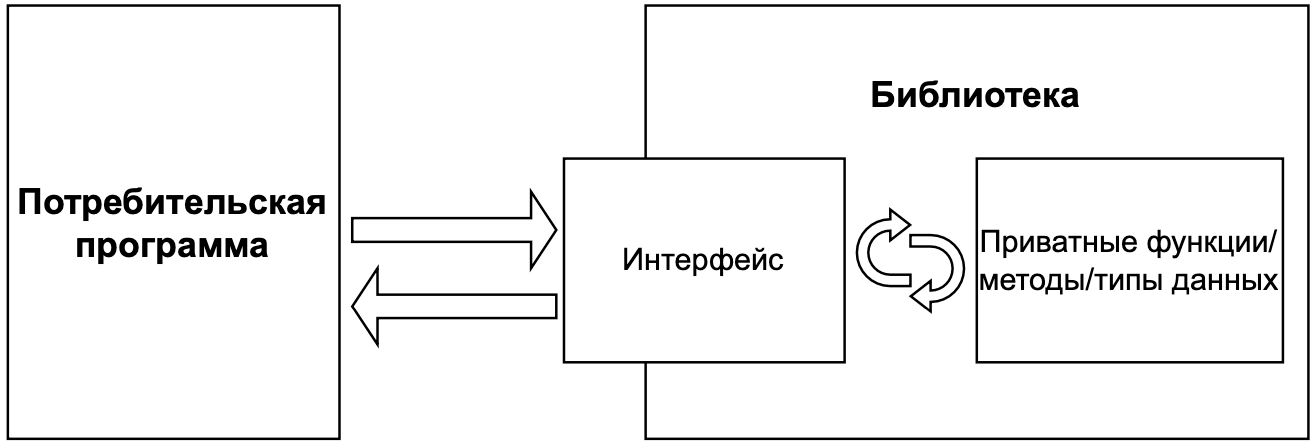
\includegraphics[scale=0.4]{LibraryInterface}
    }
    \caption{Взаимодействия между библиотекой и программой.}\label{fig:LibraryInterface}
\end{figure}

На листинге ~\cref{lst:exampleFuzzingLibpurple} показывается простая фаззинг-обертка функции purple\_utf8\_salvage в библиотеке libpurple. 

\begin{lstlisting}[language=C++,frame=single,caption={Простой пример фаззинг-обертки},label=lst:exampleFuzzingLibpurple]
#include "libpurple/util.h"
#include <stdint.h>
#include <stdlib.h>
#include <string.h>

extern "C" int LLVMFuzzerTestOneInput(const uint8_t *Data, size_t Size) 
{
    char *foo;
    foo = (char *)malloc(Size + 1);
    memcpy(foo, Data, Size);
    foo[Size] = 0;

    char *tmp  = purple_utf8_salvage(foo);
    if (tmp == 0) {
        free(foo);
        return 0;
    }
    return 0;
}\end{lstlisting} 

Результатом автоматической генерации фаззин-оберток в третей и четвертой главе является фаззинг-обертка такого типа, которая состоит из нескольких частей:
\begin{itemize}
    \item строки 1-4: включаются заголовочные файлы, содержащие определения функций, типов данных библиотеки;
    \item 6я строка: объявляется функция LLVMFuzzerTestOneInput, которая получает входной буфер фаззинга от libFuzzer;
    \item строки 8-11: объявляется переменная foo строкового типа, присваивается значение из буфера "Data";
    \item 12я строка: вызывается целевой функции с аргументом foo;
    \item строки 14-17: освобождается выделенная память;
    \item 18я строка: завершается фаззинг-обертка.
\end{itemize}

После оформления необходимо фаззинг-обертку  компилировать и линковать  с собранными динамическими или статическими файлами библиотеки. Информация о заголовочных файлах, параметрах компиляции и файлах при линковки можно получить из результата статического анализа. 

В разделе 1.2 описывается инструмент FUDGE - инструмент для генерации фаззинг-оберток для библиотеки. В 2019 году компания Google представяет инструмент FUDGE, который помогает генерировать фаззинг-оберток для билиотек. FUDGE предоставляет графический пользовательский интерфейс, который упрощает процесс создания, управления и анализа результатов работы фаззинг-оберток. FUDGE способно генерировать тесты на основе отзывов о предыдущих тестах.

Процесс генерации фаззинг-обертки в FUDGE состоит из нескольких шагов:
\begin{itemize}
    \item слайсинг (агл. slicing) - FUDGE сканирует код библиотеки, использующей целевую библиотеку, ищет и извлекает из функций примеры использования функций целевой библиотеки. Анализируя абстрактное синтаксическое дерево программы, модуль извлекает только те части дерева, которые относятся к целевой библиотеке. Функция выбирается для анализа, если она содержит хотя бы один вызов библиотечной функции, подходящей для фаззинга: например, один из аргументов которой является буфером. Вызовы функций целевой библиотеки выбираются в качестве начальных операторов в этих функциях.
    \item анализ зависимостей по данным и по управлению: выделяются зависимые операторы. Процесс синтаксического анализа помечает выражения, содержащие неизвестные символы, определенные вне функции, такие как параметр функции, глобальная переменная, функция, определенная в другой единице трансляции, или неимпримитивные типы, определенные вне целевой библиотеки. Следующим шагом является синтез кода, который заменяет помеченные операторы в извлеченных частях кода новыми выражениями с использованием сопоставления с образцом, которые могут содержать данные из буфера, сгенерированного фаззером.
    \item генерация фаззинг-обертки и запускаются с ограничением по времени. Это позволяет отсеять бесполезные обертки, которые немедленно прекращают работу, потому что содержат тривиальные ошибки. В некоторых случаях FUDGE работает хорошо, но в больших проектах генерирует много избыточных оберток, которые нужно редактировать вручную.
\end{itemize}

В разделе 1.3 описывается инструмент FuzzGen - автоматический генератор для фаззинг-оберток. FuzzGen состоит из 3 частей. На первом этапе FuzzGen сканирует всю систему и извлекает взаимодействия с API целевой библиотеки из кода, который её использует. На втором этапе строится специальный граф Abstract API Dependence Graph (A2DG), который охватывает все правиль- ные взаимодействия с API. A2DG - направленный граф, схожий с графом потока управления, который отображает последовательности правильных вызовов API. Вершины графа - вызовы функций целевой библиотеки, реб- ра - передача управления.В ребрах дополнительно содержится информа- ция о возможных диапазонах значений параметров, что улучшает итоговую производительность. A2DG позволяет выразить сложные зависимости между компонентами API. Данная структура выделяет функции которые вызываются первыми, последними, и как функции зависят друг от друга. A2DG строится в 2 ша- га. На первом шаге строится A2DG для каждой исходной функции (main в программе, каждая функция содержащая вызов API в библиотеке) в каж- дой программе, использующей целевую библиотеку.На втором шаге, все базовые A2DG соединяются в один.
На третьем этапе работы FuzzGen создается обёртка на основе имеющегося A2DG. Вместо генерации большого числа оберток для каждого графа, FuzzGen создает одну более общую обертку , которая использует энтропию из фаззера чтобы закодировать пути вызовов функций в графе.
По сравнению с FUDGE, FuzzGen создает более объёмные, общие фаззеры, которые способны выразить сложные взаимодействия с API, по срав- нению с более короткими последовательностями, получаемыми в FUDGE. Так же FuzzGen использует для анализа несколько библиотек, использую- щих целевую, а FUDGE только одну. FuzzGen полагается на качественные примеры использования целевой библиотеки, и без них неспособен создавать эффективные обёртки для фаззинга.

В разделе 1.4 описывается инструмент IntelliGen. Данный метод анализирует все функции библиотеки, и присваивает каждый из них приоритет уязвимости, который зависит от использования в функции «опасных» операций, таких как разыменование указателя и вызов функции работы с памятью (например memcpy). Далее функции сортируются по приоритету и выбираются наиболее уязвимые. Данные функции считаются входными и для них продолжается анализ. Далее производится синтез значений аргументов данных функций в процессе выполнения. Для скалярных типов значение берется из подпоследовательности байт буфера фаззера. Для указателей выделяется па- мять без инициализации, и указателю присваивается адрес этой памяти, для массивов и структур выполняются предыдущие действия рекурсивно для каждого элемента. Код выбранных функций инструментируется, что- бы реализовать принцип ленивой инициализации памяти, когда выделен- ная память будет инициализирована, только если он позже используется. Intelligen анализирует IR целевой функции и находит из сравнений подходящие значения для параметров функции и использует эту информации при генерации параметров. Так же как и в FUDGE, полученные обёртки запускаются на ограниченное время. Таким образом в случае ошибки отфильтровываются обёртки содержащие тривиальные ошибки.
Принцип работы IntelliGen более универсальный по сравнению с сопоставлением закономерностей параметров в FUDGE и анализом функций API в существующих тестовых случаях в FuzzGen, IntelliGen может определить уязвимые функции без необходимости в дополнительной информации. Из описанных ранее методов IntelliGen наиболее эффективный: в среднем показывает лучшие результаты по количеству покрытых блоков и числу найденных путей.

В \underline{\textbf{вторая главе}} описывается метод автоматического анализа исходного программных библиотек во время компиляции. 
В разделе 2.1. проводится обзор инструментов статического анализа «CodeQL» и «Clang статический анализатор»

CodeQL - это инструмент для анализа кода, разработанный компанией Semmle, которую приобрела Microsoft в 2019 году. CodeQL позволяет производить статический анализ кода, выявлять ошибки, уязвимости и другие проблемы в исходном коде приложений. Основным преимуществом CodeQL является его способность проводить контекстно-чувствительный анализ кода, позволяющий находить дефекты и уязвимости, которые могут оставаться незамеченными при использовании других инструментов. CodeQL также позволяет создавать собственные запросы для анализа кода, что обеспечивает гибкость в работе с инструментом.
CodeQL может быть использован для анализа кода на разных языках программирования, включая C++, C\#, Java, JavaScript, Python и другие. Он интегрируется с средами разработки, такими как Visual Studio Code и GitHub, что позволяет проводить анализ кода непосредственно в процессе разработки. Использование CodeQL помогает обнаруживать проблемы в коде на ранней стадии, что может сократить время и затраты на отладку и исправление ошибок. Он также может помочь повысить качество программного обеспечения и уменьшить количество уязвимостей в коде.

Для того чтобы использовать CodeQL необходимо: 
\begin{itemize}
    \item установить CodeQL;
    \item запустить CodeQL для целевой программы, чтобы создавать кодовую базу;
    \item создавать запросы;
    \item анализировать возвращаемые результаты.
\end{itemize}
так же нужно приобретать лицензию при большему количеству запросов в кодовую базу.

Clang статический анализатор (Clang Static Analyzer) - это инструмент статического анализа кода, который предназначен для поиска ошибок и потенциальных проблем в коде, которые могут привести к сбоям в работе программы, утечкам памяти, неправильному использованию указателей и другим проблемам. С помощью Clang статического анализатора можно  создавать граф потока данных и анализировать его состояния на различных участках кода. Он поддерживает анализ как C++, так и Objective-C кода и способен обрабатывать как отдельные файлы, так и целые проекты. Благодаря тому, что Clang статический анализатор входит в состав проекта LLVM, он может запускаться во время компиляции для анализа и устанавливать другое программное обеспечение.
В рамках данной работы был выбран Clang статический анализатор для разработки автоматического анализа программного кода. 

В разделе 2.2. описываются инструменты ASTVisitor и ASTMatcher, которые входят в Clang статический анализ для анализа абстрактного синтаксического дерева \(АСД\) 

На рисунке ~\cref{fig:ClangSA} отображается схема работы Clang статического анализатора во время компиляции.
\begin{figure}[ht]
    \centerfloat{
        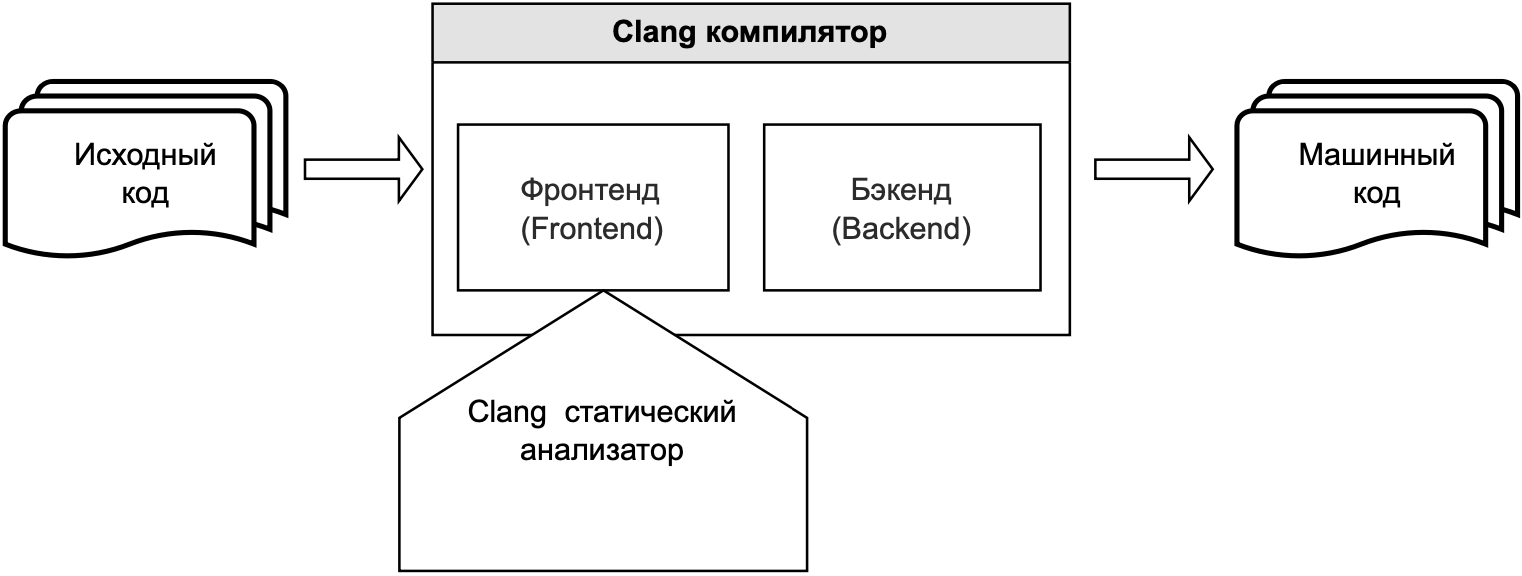
\includegraphics[scale=0.42]{ClangSA}
    }
    \caption{Схема работы статического анализатора.}\label{fig:ClangSA}
\end{figure}

АСД - это структура данных, которая представляет собой синтаксическую структуру программы в виде дерева. АСД создается в процессе компиляции или интерпретации программы и используется для упрощения анализа и обработки кода. АСД состоит из узлов дерева, которые представляют конструкции языка программирования, такие как операторы, операнды, выражения, функции и т.д. Каждый узел дерева имеет тип и может содержать ссылки на другие узлы дерева, что позволяет отображать связи между различными частями программы.

Clang статический анализатор предоставляет 2 абстрактного инструмента для анализа АСД:
\begin{itemize}
    \item {\textbf{ASTVisitor}} - это инструмент, который позволяет обходить АСД и выполнять определенные действия при посещении узлов AST. Когда ASTVisitor обнаруживает узел, который соответствует определенному типу, он вызывает соответствующую функцию-обработчик, которая выполняет необходимые действия.
    \item {\textbf{ASTMatcher}} - это инструмент, который позволяет осуществлять поиск в АСД с помощью заданных пользователем шаблонов. ASTMatcher предоставляет гибкий интерфейс для создания шаблонов с использованием DSL ( Domain Specific Language - язык предметной области), который позволяет выразить сложные критерии поиска в компактной и понятной форме. После запуска поиска по шаблонам, если находится нужные узлы функция обратного вызова MatchCallback может запускаться для обработки.
\end{itemize}

В данной работе для разных задач были разработаны разные АСД-обработчики (ASTVisitor) и АСД-детекторы (ASTMatcher), например:

Для решения задачи генерации фаззинг-оберток для функции в условиях отсутствия контекста были разработаны АСД-обработчики, которые позволяет собирать информации о сущностях кода:
\begin{itemize}
    \item определение функции: возвращаемый тип, список аргументов и их тип данных;
    \item определение перечисляемого типа: название, список констант;
    \item определение структуры, ее полей;
    \item определение класса и его атрибуты, методы;
    \item определение нового типа данных с помощью ключевого слова typedef;
    \item перечень заголовочные файлы, включенные в анализируемую единицу трансляции;
    \item параметры компиляции.
\end{itemize}
Взаимосвязи  между сущностями обнаруживаются с помощью их хэш-значения, которые являются уникальными во всем АСД.
Так же были разработаны АСД-детекторы для поиска вариантов использования аргументов функции в разных точках кода. Подробнее описывается в третьей главе.

Для решения задачи генерации фаззинг-оберток для контекста использования функций библиотеки были разработаны АСД-детекторы, которые позволяет анализировать каждое определение функции в потребительской программе. Так же были разработаны АСД-обработчики, которые строят граф поток данных и анализирует поток данных аргументов найденных вызовов. Подробнее описывается в четвертой главе.

Все разработанные инструменты запускаются одновременно с процессом сборки библиотеки или потребительской программы для упрощения участия тестирощика в анализе. Результат анализа записывается в JSON-файл, который осуществляется сохранять данные в структурированных форматах. Реализация данного процесса описывается в пятой главе.

В \underline{\textbf{Третьей главе}} описывается метод автоматической генерации фаззинг-оберток для функции в условиях отсутствия контекста использования, обсуждаются решения его основных задач:
\begin{itemize}
\item автоматическое объявление и присваивание значения из однопоточного буфера фаззера для аргументов целевой функции;
\item снижение ложных срабатываний при генерации.
\end{itemize}

В разделе 3.1. проводится обзор использования библиотеки для выделения особенностей функции, методы интерфейса. Для генерации вызов целевой функции необходимо изучать ее свойства. Как показано на рисунке~\cref{fig:LibraryInterface} существуют функции, методы являющиеся интерфейсом библиотеки, который отвечает за прием входных данных, обработку или передачу другим функциям, методам и выдачу обработанных данных обратно в потребительскую программу. В большинстве случаев входные данные передаются в библиотеку в виде фундаментальных типов, известных обям библиотеке и потребительской программе, таких как:

\begin{itemize}
    \item целые числа;
    \item десятичные дроби;
    \item логические значения;
    \item символ или строки (массив символов);
    \item файл.
\end{itemize}

В качестве примера на листинге~\cref{lst:exampleJsonC} иллюстрируется функция ipc\_event\_mode программы sway - \url{https://github.com/swaywm/sway}, которая использует библиотеку json-c для сохранения и оформления данных. В данном примере:

\begin{itemize}
    \item перед тем, как передается в функцию json\_object\_object\_add переменная obj создалась с помощью функции json\_object\_new\_object\(\);
    \item третий аргумент функции json\_object\_object\_add\(\) создается вызовом json\_object\_new\_string, который принимает строку на свой вход.
\end{itemize}

\begin{figure}[thp]
\begin{lstlisting}[language=C++,frame=single,caption={Пример использования библиотеки},label=lst:exampleJsonC]
void ipc_event_mode(const char *mode, bool pango) {
    if (!ipc_has_event_listeners(IPC_EVENT_MODE)) {
        return;
    }
    sway_log(SWAY_DEBUG, "Sending mode::%s event", mode);
    json_object *obj = json_object_new_object();
    json_object_object_add(obj, "change", 
                    json_object_new_string(mode));
    json_object_object_add(obj, "pango_markup",
                    json_object_new_boolean(pango));

    const char *json_string = json_object_to_json_string(obj);
    ipc_send_event(json_string, IPC_EVENT_MODE);
    json_object_put(obj);
}
\end{lstlisting}
\end{figure}
Функции json\_object\_object\_add и json\_object\_new\_string являются функциями интерфейсом библиотеки и называются простыми функциями в данной работе. Другие сложные функции или методы могут принимать аргументы, созданные простыми функциями библиотеки. Это важное свойство при автоматической генерации фаззинг-оберток для функции библиотеки в условиях отсутствия контекста использования.

В разделе 3.2. обсуждается метод автоматического объявления и присваивания значение из однопоточного буфера фаззера для аргументов целевой функции.
Как известно, данные из фаззера по-ступают как непрерывный единый поток данных (буфер), поэтому требуется сериализация полученных данных для передачи их аргументам функции. Минимальная длина буфера равна сумме размеров типов данных всех инициализированных аргументов. На рисунке~\cref{fig:sliceBuffer} приводится пример раз-деления буфера на части.

На приведенном примере, в сгенерированной фаззинг-обертке имеются 3 аргумента разных типов: логическое значение \(bool\) размера 1, целое число \(int\) размера 4 и строка \(char\) размера 5  из 3 элементов – тогда минимальная длина буфера равна 10.

\begin{figure}[ht]
    \centerfloat{
        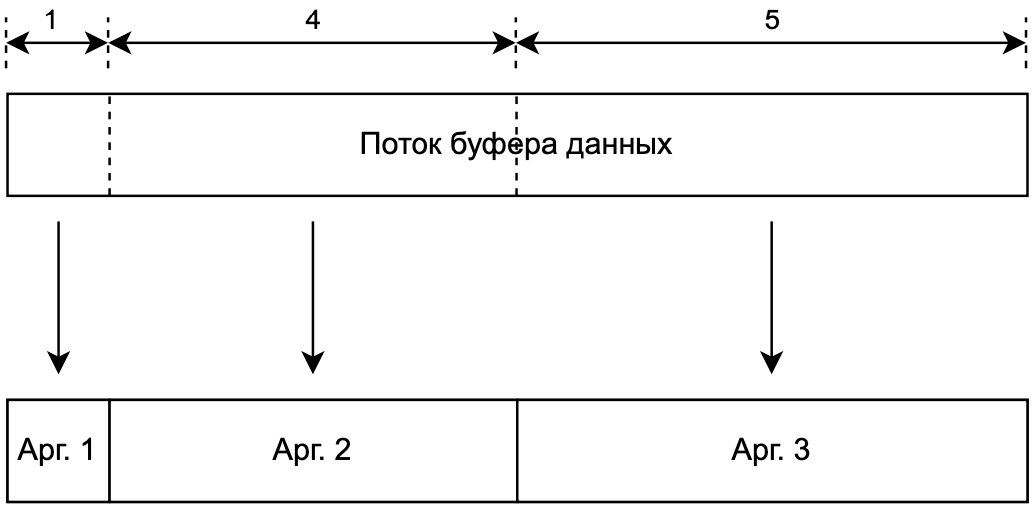
\includegraphics[scale=0.42]{sliceBuffer}
    }
    \caption{Пример разделения буфера фаззера.}\label{fig:sliceBuffer}
\end{figure}

Алгоритм~\cref{alg:algGenerationFuzzingWrapper} описывает функцию генерации фаззинг-оберток для функции в условиях отсутствия контекста использования функции. А результат метода генерации описанного в этой главе показывается на листинге ~\cref{lst:wrapperNocontext}. 

\begin{algorithm}
    \caption{Краткий алгоритм генерации фаззинг-оберток для функции в условиях отсутствия контекста}\label{alg:algGenerationFuzzingWrapper}
    \begin{algorithmic}[1]
        \Function{Генерации фаззинг-оберток}{информация о функции}
            \ForAll {аргументов}
                \If {тип данных текущего аргумента простой}
                    \State {аргумент объявляется  и присваивается значение из буфера данных фаззера}
                \Else
                    \Loop
                        \State Искать в списке простых функции библиотеки функцию, возвращающую тип данных текущего аргумента
                        \If {нашлась функция} 
                            \State {все аргументы найденной функции объявляются  и присваиваются значения из буфера данных фаззера}
                            \State текущий аргумент объявляется вызовом найденной функции с своими объявленными аргументами
                        \EndIf
                    \EndLoop
                \EndIf
            \EndFor
            \State считается минимальный размер буфер фаззера для корма аргументов
            \State включаются заголовочные файлы, полученные в процессе статического анализа единицы трансляции тестируемой функции
    \EndFunction
        \end{algorithmic}
\end{algorithm}

    Однако, существуют случаи, при которых количество ложных срабатываний значительно увеличивается:

\begin{enumerate}
    \item рассмотрим функцию json\_object\_from\_fd(int fd) в библиотеке json-c, эта функция принимает один аргумент целого типа fd. Этот аргумент на самом деле является дескриптором файла и инициализируется с помощью системного вызова open(). Передача произвольное значение данной переменной вызывается ложное срабатывание.
    \item если в качестве входных аргументов функции, передаётся строка и её размер, то т.к. значение размера зависит от предыдущей переменной (от строки) при попытке передать ей случайное значение вызывается ложное срабатывание.
    \item на листинге~\cref{lst:exampleJsonC} показан пример использования функции json\_object\_put(obj).  Эта функция принимает аргумент obj, который инициализируется функцией json\_object\_new\_object() и модифицируется функцией json\_object\_object\_add(). Таким образом, присваивание случайного значения аргументу body, нарушает контекст и вызывает ложные срабатывания.
\end{enumerate}

Для уменьшения количества ложных срабатываний при генерации фаззинг-оберток в случаях 1 и 2 необходимо анализировать варианта использования аргументов функции и в случае 3 необходимо анализировать контекст вызовов функций в других программах, библиотеках - этот анализ описывается в четвертой главе.

\begin{figure}[thp]
\begin{lstlisting}[language=C++,frame=single,caption={Результат метода генерации фаззинг-обертки в условиях отсутствия контекста использования},label=lst:wrapperNocontext]
#include "json_object.h"
#include "json_tokener.h"
#include "json_util.h"

int LLVMFuzzerTestOneInput(uint8_t * Fuzz_Data, size_t Fuzz_Size){
    if (Fuzz_Size < 1) return 0;
    size_t dyn_buffer = (size_t) (Fuzz_Size - 1);
    //generate random array of dynamic string sizes
    size_t dyn_size[1];
    dyn_size[0] = dyn_buffer;
    //end of generation random array of dynamic string sizes
    uint8_t * pos = Fuzz_Data;
    //GEN_CSTRING
    char * rstr_str = (char *) malloc(dyn_size[0] + 1);
    memset(rstr_str, 0, dyn_size[0] + 1);
    memcpy(rstr_str, pos, dyn_size[0] );
    pos += dyn_size[0];
    const char * str_str = rstr_str;
    
    //FUNCTION_CALL
    json_tokener_parse(str_str );
    //FREE
    if (rstr_str) {
        free(rstr_str);
        rstr_str = NULL;
    }
    return 0;
}
// Compile command:
/* clang -fsanitize=address,fuzzer -g -O0 -ferror-limit=1 -I. -I./.futag-build/  ./futag-drivers/json_tokener_parse1.c -o ./futag-drivers/json_tokener_parse1.out -Wl,--start-group ./.futag-build/libjson-c.a -Wl,--end-group 
 */
\end{lstlisting}
\end{figure}

В разделе 3.3. описывается метод снижения ложных срабатываний при генерации фаззинг-оберток. В листинге~\cref{lst:UsageVariant} иллюстрируется функция json\_object\_from\_file, которая принимает аргумент «fname» строкового типа «const char *». 

\begin{figure}[thp]
\begin{lstlisting}[language=C++,frame=single,caption={Пример варианта использования аргументов функции},label=lst:UsageVariant]
    struct json_object *json_object_from_file(const char *fname){
        struct json_object *obj;
        int fd;
        if ((fd = open(fname, O_RDONLY)) < 0){
            return NULL;
        }
        obj = json_object_from_fd(fd);
        close(fd);
        return obj;
    }
    \end{lstlisting}
\end{figure}

На строке 4 этот аргумент передается на вход функции open(fname, O\_RDONLY) – которая пытается открыть файл с именем, сохраняемым в переменной fname. Для того, чтобы выполнить корректный фаззинг данной функции, следует передавать в качестве значения параметра имя существующего файла. 



Контекст использования аргумента зависит от вызванной функции и его место нахождения в списке аргументов - в данной работе были разработаны АСД-детекторы для выполнения такого анализа. Перечень некоторых системных вызовов для обнаружения вариантов использования аргументов приводится в таблице~\cref{tab:ArgAnalysis}.

\begin{table}
    \centering
    \captionsetup{justification=centering}
    \caption{Перечень некоторых системных вызовов для обнаружения вариантов использования}\label{tab:ArgAnalysis}
    \begin{tabular}{|c|l|l|}
        \hline
        {1} & {open()} & Путь к файлу \\
        {2} & {fopen()} & Путь к файлу \\
        {3} & {write()} & Файловый дескриптор \\
        {4} & {close()} & Файловый дескриптор \\
        {5} & {strcpy()} & Строка, длина строки \\
        {6} & {strncpy()} & Строка, длина строки \\
        {7} & {malloc()} & длина строки, массива \\
        {8} & {memcpy()} & длина строки, массива \\
        {9} & {memset()} & длина строки, массива \\
        \hline
    \end{tabular}
\end{table}

В \underline{\textbf{четвёртой главе}} {\textbf{«Метод генерация фаззинг оберток в контексте использования»}} описывается метод вывести контекст вызовов функций тестируемой библиотеки для генерации фаззинг-оберток. Данный метод воспользуется результатом анализа во второй, в третей главе и графом потока управления, анализом поток данных для определения правильного контекста.

Граф потока управления (Control Flow Graph - ГФУ) - это графическое представление программного кода, которое показывает, как управление потоком проходит через программу. CFG отображает структуру программы, показывая последовательность операций и переходы между ними, которые могут происходить во время выполнения программы. Граф потока управления представляет программный код в виде узлов и ребер, где узлы представляют блоки кода, а ребра связывают блоки кода в порядке их выполнения. Каждый блок кода может содержать несколько операторов, которые выполняются последовательно, и переходы, которые могут произойти после выполнения блока.

Анализ потока данных (Data Flow Analysis) - это метод статического анализа программного кода, который позволяет определить потоки данных в программе и анализировать их свойства, такие как зависимости, переопределение, использование и т.д. Анализ потока данных может помочь выявить ошибки и уязвимости в программе, а также оптимизировать ее производительность.

Анализ потока данных может быть выполнен с помощью различных инструментов и методов, таких как граф потока данных (Data Flow Graph), системы типов, аннотации и т.д. Во время анализа потока данных инструменты и методы используются для поиска зависимостей между переменными, функциями и операторами в программе. Например, анализ потока данных может помочь выявить неиспользуемые переменные, неиспользуемый код, некорректные пути выполнения программы и т.д.

Был разработан АСД-обработчик, который запускается в каждом узле потребительской программе для обнаружения вызовов функций тестируемой. Если нашлись такие вызовы, другой АСД-детектор запускается для поиска зависимые вызовы, которые обрабатывают аргументов найденных вызовов. Такой анализ реализуется алгоритмом~\cref{alg:algContextAnalysis}. В результате обработки сгенерирована фаззинг-обертка на листинге~\cref{lst:lst:wrapperWContext}



\begin{algorithm}
    \caption{Алгоритм анализа контекста вызовов функций тестируемой библиотеки в других программах}\label{alg:algContextAnalysis}
    \begin{algorithmic}[1]
        \Function{Анализ контекста}{информация о тестируемой библиотеке}
            \State Запускать АСД-детектор 1 для поиска вызовов простых функций тестируемой библиотеки
            \If {нашлись вызовы {\textbf{В}}}
                \State Строить ГФУ для данной функции
                \State Искать все пути {\textbf{П}} выполнения в ГФУ
                \For {для каждого вызова {\textbf{в}} из {\textbf{В}}}
                    \State добавлять {\textbf{в}} в контекст {\textbf{К}}
                    \State запускать АСД-детектор 2 для поиска вызовов, зависящие от выбранного вызова
                    \If {нашлись вызовы {\textbf{М}}}
                        \ForAll {вызовов из {\textbf{М}}}
                            \State определять к какому блоку принадлежит найденные вызовы, этот блок добавляется в список блоков {\textbf{Б}}
                            \State определять способ оформления аргументов вызова: константа, объявленная переменная или вызов другой функции
                            \If {аргумент вызова {\textbf{М}} - переменная, объявленная с помощью простой функции в тестируемой библиотеки}
                                \State добавлять вызов в контекст {\textbf{К}}
                            \EndIf
                            \If {аргумент вызова {\textbf{М}} - константа}
                                \State добавлять константу в контекст {\textbf{К}}
                            \EndIf
                            \If {аргумент вызова {\textbf{М}} - вызов другой функции {\textbf{Ф}} в тестируемой библиотеки}
                                \State заменять этот вызов новой переменной {\textbf{E}}, которая объявляется вызовом {\textbf{Ф}}
                                \State добавлять {\textbf{E}} и {\textbf{Ф}} в контекст {\textbf{К}}
                            \EndIf
                        \EndFor
                        \State добавлять путь, к которому принадлежат блоки {\textbf{Б}} в контекст {\textbf{К}}
                    \EndIf
                \EndFor
            \EndIf
        \EndFunction
    \end{algorithmic}
\end{algorithm}

\begin{figure}[thp]
    \begin{lstlisting}[language=C++,frame=single,caption={Результат метода генерации фаззинг-обертки c контекстом использования},label=lst:wrapperWContext]
#include "json.h"

int LLVMFuzzerTestOneInput(uint8_t * Fuzz_Data, size_t Fuzz_Size){
    if (Fuzz_Size < 2) return 0;
    size_t dyn_buffer = (size_t) ((Fuzz_Size - 2));
    //generate random array of dynamic string sizes
    size_t dyn_size[2];
    srand(time(NULL));
    dyn_size[0] = rand() % dyn_buffer;
    size_t remain = dyn_size[0];
    for(size_t i = 1; i< 2 - 1; i++){
        dyn_size[i] = rand() % (dyn_buffer - remain);
        remain += dyn_size[i];
    }
    dyn_size[1] = dyn_buffer - remain;
    //end of generation random array of dynamic string sizes
    uint8_t * pos = Fuzz_Data;

    struct json_object *body = json_object_new_object();

    //GEN_CSTRING
    char * rstr_str0 = (char *) malloc(dyn_size[0] + 1);
    memset(rstr_str0, 0, dyn_size[0] + 1);
    memcpy(rstr_str0, pos, dyn_size[0] );
    pos += dyn_size[0];
    const char * str_str0 = rstr_str0;

    struct json_object *FutagRefVarueK = json_object_new_string(str_str1);
    json_object_object_add(body, "dataHash", FutagRefVarueK);

    //GEN_CSTRING
    char * rstr_str1 = (char *) malloc(dyn_size[1] + 1);
    memset(rstr_str1, 0, dyn_size[0] + 1);
    memcpy(rstr_str1, pos, dyn_size[0] );
    pos += dyn_size[0];
    const char * str_str1 = rstr_str1;

    struct json_object *FutagRefVar73q = json_object_new_string(str_str1);
    json_object_object_add(body, "token", FutagRefVar73q);

    json_object_put(body);
    return 0;
}
// Compile command:
/* 
clang -fsanitize=address,fuzzer -g -O0 -ferror-limit=1 -I. -I./.futag-build/  ./futag-drivers/context1.c -o ./futag-drivers/context1.out -Wl,--start-group ./libjson-c.a -Wl,--end-group
*/
\end{lstlisting}
\end{figure}

В \underline{\textbf{пятой главе}} {\textbf{«Реализация предложенных методов в программных инструментах»}} описана реализация методов программным продуктом, который позволяет:
\begin{itemize}
    \item автоматически анализировать тестируемую библиотеку во время ее компиляции;
    \item автоматически генерировать и компилировать фаззинг-обертки в двух условиях: с и без контекстом использования тестируемой библиотеки;
    \item автоматически фаззить скомпилированные фаззинг-обертки, анализировать результат фаззинга и выдавать пользователям отчет в формате SVACE или лог-файла.
\end{itemize}.

Программный продукт с названием Futag опубликован в GitHub по адресу \url{http://github.com/ispras/Futag/}, который содержит:
\begin{itemize}
    \item модифицируемый проект LLVM с набором инструментов: компилятор clang, clang++, датчиками обнаружения ошибок AddressSanitizer и т.д.;
    \item АСД-обработчики и АСД-детекторы;
    \item Python-пакет, который позволяет управлять процесс компиляции тестируемой библиотеки, автоматически генерировать фаззинг-обертки с помощью простого скрипта на листинге~\cref{lst:testScript}.
\end{itemize}.
\begin{figure}[thp]
    \begin{lstlisting}[language=Python,frame=single,caption={Скрипт для запуска инструмент Futag},label=lst:testScript]
from futag.preprocessor import *
from futag.generator import *
from futag.fuzzer import *

testing_lib = Builder(
    "futag-llvm/", # path to Futag package
    "path/to/library/source/code" 
)
testing_lib.auto_build() # build automatically
testing_lib.analyze() # analyze the information

g = Generator(
    "futag-llvm/", # path to Futag package
    "path/to/library/source/code" 
)
g.gen_targets() # Generate fuzz drivers
g.compile_targets() # Compile fuzz drivers

fuzzer = Fuzzer(
    "futag-llvm/", # path to Futag package
    "futag-fuzz-drivers", #contains fuzz-targets
    fork=4,  
    totaltime=60,
    gdb=True,
)
fuzzer.fuzz()        
\end{lstlisting}
\end{figure}
После запуска скрипта Futag проводит следующие действия:
- компилирует исследуемую библиотеку с датчиками обнаружения ошибок (AddressSanitizer) и собирает информации о параметрах команд компиляции;
- инициализирует библиотеку в пространстве пользователя ОС, для сбора информации о заголовочных файлах и статических библиотеках, использованных в процессе компиляции;
- генерирует и компилирует фаззинг-обертки;
- запускает скомпилированные фаззинг-обертки и собирает результат фаззинга;
- результат фаззинга автоматически обрабатывается отладчиком GDB для сбора информации о переменных в месте ошибки.


\FloatBarrier
\pdfbookmark{Заключение}{conclusion}                                  % Закладка pdf
В \underline{\textbf{заключении}} приведены основные результаты работы, которые заключаются в следующем:
%% Согласно ГОСТ Р 7.0.11-2011:
%% 5.3.3 В заключении диссертации излагают итоги выполненного исследования, рекомендации, перспективы дальнейшей разработки темы.
%% 9.2.3 В заключении автореферата диссертации излагают итоги данного исследования, рекомендации и перспективы дальнейшей разработки темы.
\begin{enumerate}
  \item Разработан метод автоматического генерации фаззинг-оберток для функций библиотеки в условиях отсутствия контекста использования. Для снижения количество ложных срабатываний был разработан детектор, который позволяет обнаруживать вариант использования аргументов тестируемой функции.  \ldots
  \item Разработан метод автоматического генерации фаззинг-оберток для функций библиотеки с учетом контекста использования. Данный метод заключается в анализе графа потока управления и потока данных для обнаружения контекст вызовов тестируемой библиотеки в потребительских программах.  \ldots
  \item Разработан программный продукт, который полностью автоматизирует процесс тестирования программных библиотек с применением статического и динамического анализов.
\end{enumerate}


\pdfbookmark{Литература}{bibliography}                                % Закладка pdf

\ifdefmacro{\microtypesetup}{\microtypesetup{protrusion=false}}{} % не рекомендуется применять пакет микротипографики к автоматически генерируемому списку литературы
\urlstyle{rm}                               % ссылки URL обычным шрифтом
\ifnumequal{\value{bibliosel}}{0}{% Встроенная реализация с загрузкой файла через движок bibtex8
    \renewcommand{\bibname}{\large \bibtitleauthor}
    \nocite{*}
    \insertbiblioauthor           % Подключаем Bib-базы
    %\insertbiblioexternal   % !!! bibtex не умеет работать с несколькими библиографиями !!!
}{% Реализация пакетом biblatex через движок biber
    % Цитирования.
    %  * Порядок перечисления определяет порядок в библиографии (только внутри подраздела, если `\insertbiblioauthorgrouped`).
    %  * Если не соблюдать порядок "как для \printbibliography", нумерация в `\insertbiblioauthor` будет кривой.
    %  * Если цитировать каждый источник отдельной командой --- найти некоторые ошибки будет проще.
    %
    %% authorvak
    \nocite{scbib1}%conf
    \nocite{bib1}%conf
    \nocite{confbib1}%conf
    \nocite{confbib2}%conf
    \nocite{bib2}%conf
    %

    \ifnumgreater{\value{usefootcite}}{0}{
        \begin{refcontext}[labelprefix={}]
            \ifnum \value{bibgrouped}>0
                \insertbiblioauthorgrouped    % Вывод всех работ автора, сгруппированных по источникам
            \else
                \insertbiblioauthor      % Вывод всех работ автора
            \fi
        \end{refcontext}
    }{
        \ifnum \totvalue{citeexternal}>0
            \begin{refcontext}[labelprefix=A]
                \ifnum \value{bibgrouped}>0
                    \insertbiblioauthorgrouped    % Вывод всех работ автора, сгруппированных по источникам
                \else
                    \insertbiblioauthor      % Вывод всех работ автора
                \fi
            \end{refcontext}
        \else
            \ifnum \value{bibgrouped}>0
                \insertbiblioauthorgrouped    % Вывод всех работ автора, сгруппированных по источникам
            \else
                \insertbiblioauthor      % Вывод всех работ автора
            \fi
        \fi
        %  \insertbiblioauthorimportant  % Вывод наиболее значимых работ автора (определяется в файле characteristic во второй section)
        \begin{refcontext}[labelprefix={}]
            \insertbiblioexternal            % Вывод списка литературы, на которую ссылались в тексте автореферата
        \end{refcontext}
        % Невидимый библиографический список для подсчёта количества внешних публикаций
        % Используется, чтобы убрать приставку "А" у работ автора, если в автореферате нет
        % цитирований внешних источников.
        \printbibliography[heading=nobibheading, section=0, env=countexternal, keyword=biblioexternal, resetnumbers=true]%
    }
}
\ifdefmacro{\microtypesetup}{\microtypesetup{protrusion=true}}{}
\urlstyle{tt}                               % возвращаем установки шрифта ссылок URL
